\documentclass{standalone}

\usepackage{standalone}
\usepackage{tikz}
\usetikzlibrary{er,positioning, calc}

\begin{document}

    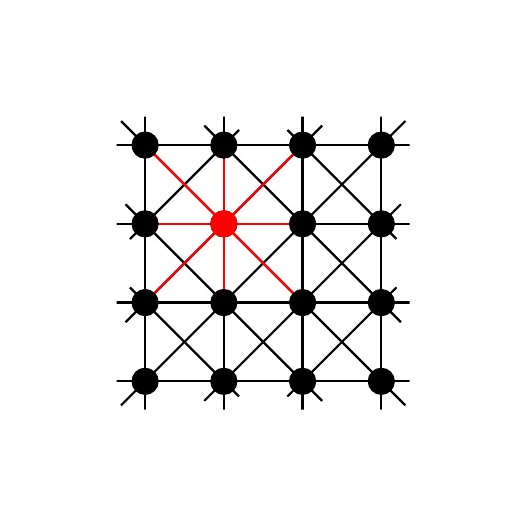
\begin{tikzpicture}
        \tikzstyle{state}=[minimum width=0.1cm, font=\boldmath];

        \node[circle, draw=black, fill=black] (0) at (0, 0) [state] {};
        \node[circle, draw=black, fill=black] (1) at (1, 0) [state] {};
        \node[circle, draw=black, fill=black] (2) at (0, -1) [state] {};
        \node[circle, draw=black, fill=black] (3) at (1, -1) [state] {};

        \node[circle, draw=black, fill=black] (4) at (1, 1) [state] {};
        \node[circle, draw=black, fill=black] (5) at (0, 1) [state] {};
        \node[circle, draw=black, fill=black] (6) at (0, -2) [state] {};
        \node[circle, draw=black, fill=black] (7) at (1, -2) [state] {};

        \node[circle, draw=black, fill=black] (8) at (-1, 0) [state] {};
        \node[circle, draw=black, fill=black] (9) at (2, 0) [state] {};
        \node[circle, draw=black, fill=black] (10) at (2, -1) [state] {};
        \node[circle, draw=black, fill=black] (11) at (-1, -1) [state] {};

        \node[circle, draw=black, fill=black] (12) at (-1, 1) [state] {};
        \node[circle, draw=black, fill=black] (13) at (2, 1) [state] {};
        \node[circle, draw=black, fill=black] (14) at (-1, -2) [state] {};
        \node[circle, draw=black, fill=black] (15) at (2, -2) [state] {};

        \draw (4) edge[out=90, in=-90, -, thick, black] node {} (7);
        \draw (5) edge[out=90, in=-90, -, thick, black] node {} (6);
        \draw (8) edge[out=180, in=0, -, thick, black] node {} (9);
        \draw (10) edge[out=0, in=-180, -, thick, black] node {} (11);

        \draw (14) edge[out=-90, in=90, -, thick, black] node {} (12);
        \draw (13) edge[out=90, in=-90, -, thick, black] node {} (15);
        \draw (14) edge[out=180, in=0, -, thick, black] node {} (15);
        \draw (12) edge[out=180, in=0, -, thick, black] node {} (13);

        \draw (12) edge[out=135, in=-45, -, thick, black] node {} (15);
        \draw (13) edge[out=45, in=-135, -, thick, black] node {} (14);
 
        \draw (11) edge[out=-135, in=45, -, thick, black] node {} (4);
        \draw (6) edge[out=-135, in=45, -, thick, black] node {} (9);

        \draw (5) edge[out=135, in=-45, -, thick, black] node {} (10);
        \draw (8) edge[out=135, in=-45, -, thick, black] node {} (7);

        \draw (5) edge[out=45, in=-135, -, thick, black] node {} (8);
        \draw (4) edge[out=135, in=-45, -, thick, black] node {} (9);

        \draw (11) edge[out=135, in=-45, -, thick, black] node {} (6);
        \draw (7) edge[out=-135, in=45, -, thick, black] node {} (10);

        \node[circle, draw=red, fill=red] (0) at (0, 0) [state] {};
        \draw (0) edge[out=90, in=-90, -, thick, red] node {} (5);
        \draw (0) edge[out=-90, in=90, -, thick, red] node {} (2);
        \draw (0) edge[out=180, in=0, -, thick, red] node {} (8);
        \draw (0) edge[out=0, in=180, -, thick, red] node {} (1);
        \draw (12) edge[out=-45, in=135, -, thick, red] node {} (3);
        \draw (11) edge[out=45, in=-135, -, thick, red] node {} (4);
    \end{tikzpicture}
\end{document}